\documentclass[11pt,letterpaper]{article}

% ---------------------------------------------------------------------------
% Explanation is not certification
% Chelsea McElveen, LogNovations Holdings LLC
% ---------------------------------------------------------------------------

\usepackage[utf8]{inputenc}
\usepackage[T1]{fontenc}
\usepackage{lmodern}
\usepackage{microtype}
\usepackage[margin=1in]{geometry}
\usepackage{amsmath,amssymb,amsthm,mathtools,bm}
\usepackage{graphicx}
\usepackage{booktabs}
\usepackage{caption}
\usepackage{enumitem}
\usepackage{xcolor}
\usepackage{tikz}
\usetikzlibrary{arrows.meta,positioning,calc}
\usepackage[numbers,sort&compress]{natbib}
\usepackage[colorlinks=true,linkcolor=blue!50!black,citecolor=blue!50!black,urlcolor=blue!50!black]{hyperref}
\usepackage{doi}
\usepackage{url}
\def\UrlBreaks{\do\/\do-\do_\do.}

\captionsetup{font=small,labelfont=bf,width=0.95\textwidth}
\setlist{nosep}

% --- macros ---------------------------------------------------------------
\newcommand{\sem}[1]{[\![#1]\!]}
\newcommand{\X}{\mathcal{X}}
\newcommand{\Y}{\mathcal{Y}}
\newcommand{\Lang}{\mathcal{L}}
\newcommand{\LU}{\Lang_{U}}
\newcommand{\D}{D}
\newcommand{\R}{\mathbb{R}}
\newcommand{\N}{\mathbb{N}}
\newcommand{\E}{\mathbb{E}}
\renewcommand{\Pr}{\mathbb{P}}
\newcommand{\ind}[1]{\mathbf{1}[#1]}
\DeclareMathOperator{\ECS}{ECS}
\DeclareMathOperator{\TV}{TV}
\DeclareMathOperator{\UCB}{UCB}
\DeclareMathOperator{\err}{err}
\DeclareMathOperator{\Unif}{Unif}
\DeclareMathOperator{\Bin}{Bin}
\DeclareMathOperator*{\argmax}{arg\,max}
\newcommand{\cz}{c_{0}}
\newcommand{\co}{c_{1}}
\newcommand{\tauhat}{\hat{\tau}}
\newcommand{\Ltwo}{\log_{2}}

\theoremstyle{plain}
\newtheorem{theorem}{Theorem}
\newtheorem{lemma}{Lemma}
\newtheorem{proposition}{Proposition}
\newtheorem{corollary}{Corollary}
\theoremstyle{definition}
\newtheorem{definition}{Definition}
\theoremstyle{remark}
\newtheorem{remark}{Remark}

\title{\LARGE\bfseries Explanation is not certification:\\[2pt]
\Large information-theoretic limits of interpretability-based assurance\\ for machine learning systems}

\author{Chelsea McElveen\\[2pt]
\small LogNovations Holdings LLC, San Francisco, CA, USA\\
\small \texttt{chelsea.anne.mcelveen@gmail.com}}

\date{\small 2 November 2026 \quad$\cdot$\quad Preprint, version 1}

\begin{document}
\maketitle

\begin{abstract}
\noindent
Regulated deployments of machine learning keep a human reviewer in the loop because no one can certify a model's outputs from the outside. The hope that interpretability will remove the reviewer, that outputs can be certified once the model's computation can be seen, is widely held. We give it a formal test. An explanation is a two-part code for a model's behaviour on an audit set, scored by the bits it saves, and five limits follow. The model offered as its own explanation has non-positive gain on any audit smaller than itself, and its transmitted internal state has negative gain always. No fixed budget covers all behaviours, so every fixed-budget standard contains an unavoidable defer outcome. The optimal score is uncomputable, so a checkable standard must fix a decidable explanation language. Faithfulness and correctness are independent, so an explanation never replaces a specification or a label. A chain of thought has negative gain and, where tested, omits an inserted cause on most of the inputs where that cause changed the output; an attribution graph with the model's attention patterns frozen in is a second model, not an explanation. What can be certified is a finite-sample bound on the error rate among auto-accepted outputs, from any score fixed in advance and an i.i.d.\ calibration sample. The guarantee does not depend on interpretability; within it, an explanation residual is worth exactly the human reviews it removes. Simulations confirm the bound and locate its hypotheses. We draw the implications for the EU AI Act, model-risk guidance and aviation standards, and pre-register the experiment that measures whether an explanation residual adds coverage.
\end{abstract}

\section{Introduction}

A model whose outputs are good is not yet a model whose outputs can be used. In credit, insurance, health, aviation and defence, a learned system's decisions are reviewed by people before they take effect, because the deployer must be able to show a regulator why a decision was acceptable, and a statistical track record is not an account of any particular decision. The European Union's Artificial Intelligence Act requires human oversight of high-risk systems (Article~14) and transparency sufficient for deployers to interpret a system's output (Article~13) \citep{euaiact2024}; United States model-risk guidance asks banks to establish the conceptual soundness of a model and to analyse its outcomes \citep{sr117}; the European aviation regulator's guidance for machine learning makes explainability a core requirement \citep{easa2024}. In these settings the human reviewer is the cost of compliance, and the cost is large: each output is read by a person before it is relied on.

The hope that interpretability will remove the reviewer is natural and widely held. If one could see the steps a model took to reach an output, the argument goes, one could certify the output the way an auditor certifies a derivation. Mechanistic interpretability has made that hope concrete. Attribution graphs now trace, for a single prompt, which learned features contributed to a model's next-token decision \citep{ameisen2025circuit,lindsey2025biology}; the tools are open \citep{anthropic2025opensource}; the field was named a breakthrough technology of 2026 \citep{mittechreview2026}. Reasoning models write out a chain of thought that reads like a derivation.

Two recent observations sharpen the question. The first is Hinton's account of what understanding is in a language model: ``very unlike translating into some special internal language and much more like folding a protein'' \citep{hinton2026vienna}. On that picture, as we read it, each word's representation is adjusted until every constraint is satisfied by every other, so the only complete account of an output is the settled state itself, and there is no derivation to audit. Hinton did not offer the fold as a certification device; the inference is ours, and Section~\ref{sec:limits} makes it precise. The second is the measured unfaithfulness of chains of thought: on inputs where an inserted hint demonstrably changed a reasoning model's answer, the chain of thought mentioned the hint on average 25\% of the time for one frontier model and 39\% for another \citep{chen2025reasoning}.

This paper asks what an explanation can certify, in principle, and answers with proofs. Our contributions are the following.

\begin{enumerate}[leftmargin=1.6em]
\item \textbf{A formal notion of explanation as compression.} An explanation of a model's behaviour on an audit set is a two-part code: a description of length $\ell(E)$ plus the bits needed to correct it where it is wrong (Section~\ref{sec:setting}). The score is the bits saved relative to transmitting the outputs with no explanation. The construction is the minimum description length principle \citep{rissanen1978,grunwald2007} with the model as the data; the same two quantities, length and residual, are what recent interpretability work measures as proof length and bound tightness \citep{gross2024} and as description length of feature dictionaries \citep{ayonrinde2024}.
\item \textbf{Five limits} (Section~\ref{sec:limits}). (i) The model itself, offered as its explanation, has non-positive gain on any audit set smaller than the model's description, and its literal internal state has negative gain always (Theorem~\ref{thm:selfref}, Corollary~\ref{cor:state}). (ii) For every explanation language and budget, most behaviour tables have no faithful explanation within budget, so a fixed-budget standard must contain a defer outcome (Theorem~\ref{thm:counting}). (iii) The optimal explanation score is uncomputable, so a checkable standard must fix a decidable explanation language (Theorem~\ref{thm:uncomputable}). (iv) The faithfulness of an explanation and the correctness of the model's outputs are independent, so an explanation can never substitute for a specification or a label (Theorem~\ref{thm:independence}). (v) A chain of thought is a per-input explanation with negative gain and, where its faithfulness has been measured, a large interventional residual (Proposition~\ref{prop:cot}).
\item \textbf{What can be certified} (Section~\ref{sec:certify}). With any score fixed in advance and an i.i.d.\ calibration sample, a finite-sample bound on the error rate among auto-accepted outputs, holding with probability $1-\delta$ (Theorem~\ref{thm:selective}). The machinery is classical \citep{geifman2017,bates2021rcps,angelopoulos2021ltt}; we restate it because our point is what it does not depend on. The guarantee is the same for a random score and for a perfect explanation; only the fraction of outputs that can be accepted changes. Within this certificate an explanation residual is therefore worth exactly the human reviews it removes at a fixed certified risk (Proposition~\ref{prop:value}), and a chain of checkers must end in a trusted base outside the learned stack (Proposition~\ref{prop:regress}).
\item \textbf{Simulations and a pre-registered experiment} (Sections~\ref{sec:simulation} and~\ref{sec:experiment}). Simulations with known ground truth confirm the bound, show that it is conservative, and show that one of its hypotheses, a grid fixed independently of the sample, cannot be dropped. The empirical question this paper leaves open, whether an explanation residual raises certified coverage over cheap uncertainty scores, is reduced to a single measurement, which we pre-register with predicted outcomes. Applied to attribution graphs (Section~\ref{sec:instantiation}), the accounting sorts their components: a per-prompt graph with the model's attention patterns frozen in, over a dictionary trained on the model, is a second model rather than an explanation; the rules distilled from many graphs can be explanations; and the graph's residuals are scores.
\end{enumerate}

The results are stated for finite input and output sets so that every count is exact; Theorem~\ref{thm:uncomputable} needs a countably infinite input set. Full proofs are in Appendix~\ref{app:proofs}. The conclusion for regulation is in Section~\ref{sec:regulation}: explanations can be required, but they cannot be required to exist, and a requirement to explain must name the language in which the explanation is to be given.

\section{An explanation is a code}
\label{sec:setting}

Logarithms are base 2. Let $\X$ be a finite input set and $\Y$ a finite output set with $q := |\Y| \ge 2$, and let $\Delta(\Y)$ be the probability distributions on $\Y$. A \emph{model} is a map $M:\X\to\Delta(\Y)$, written $M(y\mid x)$; a deterministic model is the point-mass case, written $M(x)\in\Y$.

An \emph{explanation language} is a pair $(\Lang,\sem{\cdot})$ where $\Lang\subset\{0,1\}^{*}$ is prefix-free and $\sem{\cdot}:\Lang\to(\X\to\Delta(\Y))$ is computable. The length of an explanation is $\ell(E):=|E|$ bits. The \emph{universal language} $\LU$ is the set of programs for a fixed universal prefix machine $U$ that halt on every $x\in\X$ and output a distribution on $\Y$, with $\sem{E}(x)$ that distribution.

\paragraph{Side-information rule.} The semantics $\sem{\cdot}$ is fixed before, and independently of, the model being explained. An explanation may depend on the input $x$ and on its own string, and on nothing else: any dependence on the model's internal state $z(x)$ (activations, attention patterns, weights, ``the fold''), and any model-specific component of the machinery that reads an explanation (a feature dictionary trained on the model, a readout), must be carried inside $E$ and paid for in $\ell(E)$. Nothing is free because it is already inside the system. By the invariance theorem, any language that obeys the rule embeds in the universal language at a constant additive cost, which is why Theorem~\ref{thm:selfref} is stated there; without the rule, a one-bit ``explanation'' whose semantics is the model itself would score perfectly, and the scores below would measure nothing.

\paragraph{Correction cost.} Fix a rational $\eta\in(0,1)$ (any computable $\eta$ would do) and define the smoothed prediction $\sem{E}_{\eta}(\cdot\mid x):=(1-\eta)\sem{E}(\cdot\mid x)+\eta\,\Unif(\Y)$ and the per-input correction cost
\begin{equation}
c_{\eta}(y\mid E,x) := -\Ltwo \sem{E}_{\eta}(y\mid x)\in[\cz,\co],\qquad
\cz:=\Ltwo\frac{1}{1-\eta+\eta/q}>0,\quad \co:=\Ltwo\frac{q}{\eta}.
\label{eq:cost}
\end{equation}
This is the number of bits an arithmetic coder needs to transmit the model's actual output $y$ given the explanation's prediction, up to a two-bit constant per sequence that we ignore. Smoothing keeps the cost finite when a deterministic explanation is wrong; its price is the agreement cost $\cz$, paid even when the explanation is right.

\begin{definition}[two-part code, gain, score]
\label{def:ecs}
Let $\D=((x_1,y_1),\dots,(x_n,y_n))$ be an \emph{audit set}, $y_i$ the model's observed output on $x_i$. The \emph{code length} of $E$ on $\D$, the \emph{null length}, the \emph{gain} and the \emph{explanation compression score} are
\begin{align}
L_{\D}(E) &:= \ell(E)+\sum_{i=1}^{n}c_{\eta}(y_i\mid E,x_i),\qquad
L_{\D}(\varnothing):=n\Ltwo q,\\
G_{\D}(E) &:= L_{\D}(\varnothing)-L_{\D}(E),\qquad\qquad\ \ \,
\ECS_{\D}(E):=\frac{G_{\D}(E)}{L_{\D}(\varnothing)}\le 1.
\end{align}
\end{definition}

A score above 0 means the explanation compresses the model's behaviour on $\D$; at or below 0, it does not.

\begin{definition}[residual]
\label{def:residual}
For deterministic $M$ let $\hat y_E(x):=\argmax_{y}\sem{E}(y\mid x)$ with a fixed tie rule, whether or not $\sem{E}$ is deterministic, and $r_E(x):=\ind{\hat y_E(x)\neq M(x)}$. For general $M$, $r_E(x):=\TV(M(\cdot\mid x),\sem{E}(\cdot\mid x))$. The mean residual is $R_{\D}(E):=\frac1n\sum_i r_E(x_i)$, and $E$ is \emph{$\varepsilon$-faithful} on $\D$ when $R_{\D}(E)\le\varepsilon$.
\end{definition}

\begin{lemma}[code length is length plus a per-error charge]
\label{lem:identity}
If $M$ and $\sem{E}$ are deterministic and $k:=nR_{\D}(E)$ is the number of disagreements on $\D$, then
$\sum_{i=1}^{n}c_{\eta}(y_i\mid E,x_i)=(n-k)\cz+k\co$.
\end{lemma}

Lemma~\ref{lem:identity} is the accounting identity that the rest of the paper rests on: an explanation plus its residual, priced in bits, equals the behaviour. Everything in this section is standard; it is the common ground on which the limits below are stated. The pair (length, residual) is what \citet{gross2024} measure as proof length and bound tightness, what causal scrubbing \citep{chan2022scrubbing} measures as hypothesis and loss recovered, and what \citet{ayonrinde2024} minimise as description length.

\section{Five limits}
\label{sec:limits}

\subsection{The model is not its own explanation on any audit smaller than itself}

Let $K_U(M):=\min\{|E|:E\in\LU,\ \sem{E}=M\}$ be the length of a shortest program for the model.

\begin{theorem}[self-reference]
\label{thm:selfref}
Let $E_M\in\LU$ be any explanation with $\sem{E_M}=M$. Then
\begin{equation}
G_{\D}(E_M)\ \le\ n\,(\Ltwo q-\cz)-K_U(M).
\end{equation}
In particular $G_{\D}(E_M)\le 0$, hence $\ECS_{\D}(E_M)\le 0$, whenever $n\le K_U(M)/(\Ltwo q-\cz)$, with strict inequality below that threshold.
\end{theorem}

\begin{corollary}[the settled state, transmitted literally, is not an explanation]
\label{cor:state}
Let $E_z$ carry the model's internal state $z(x_i)$ for each audited input literally, as a fixed-width record of $w$ bits, and apply the model's readout. Then $G_{\D}(E_z)\le n(\Ltwo q-\cz-w)-\ell(\mathrm{readout})$, which is negative for every $n$ as soon as $w>\Ltwo q$.
\end{corollary}

\begin{remark}[large audits]
\label{rem:large}
For deterministic $M$ every explanation pays at least $n\cz$ in corrections, so $\ECS_{\D}(E)\le 1-\cz/\Ltwo q$ for every $E$, and $E_M$ attains $1-\cz/\Ltwo q-K_U(M)/(n\Ltwo q)$. As $n$ grows with $M$ fixed, the model becomes an optimal explanation of its own behaviour. Explanation is relative to the size of what is explained; the model is penalised as its own explanation exactly when the audit is smaller than the model, which is the regime of every real audit: a calibration sample of $10^{3}$ to $10^{6}$ outputs against a model whose shortest description is of order $10^{10}$ bits (the parameter count bounds $K_U(M)$ only from above; lossless compression of trained weights without behavioural change is rarely better than about tenfold).
\end{remark}

Theorem~\ref{thm:selfref} follows from the definitions; we state it because it is the formal content of the objection that conditional Kolmogorov complexity $K(x\mid x)=O(1)$ holds for noise and for a proof alike: conditioning on the state hides the bill. Hinton's fold, offered as the account of an output, is worthless as an explanation of any audit smaller than the model, because referencing the state costs the state. An explanation earns a positive score only by being shorter than what it explains, which is the whole content of the word. A residual stream of 32 layers and width 4096 at 16 bits is $w\approx 2.1\times10^{6}$ bits per input against at most 17 bits of output for a vocabulary of $2^{17}$; Corollary~\ref{cor:state} applies with room to spare.

\subsection{No fixed budget covers all behaviours}

\begin{theorem}[no universal explainer]
\label{thm:counting}
Fix a prefix-free language $\Lang$, a budget $\ell\ge0$, a tolerance $0\le\varepsilon<\tfrac12$ (also $\varepsilon=\tfrac12$ when $q\ge3$) and $n$ distinct audit inputs. Of the $q^{n}$ behaviour tables $t\in\Y^{n}$ on these inputs, the number admitting some $E\in\Lang$ with $|E|\le\ell$ and 0-1 residual $R_{\D}(E)\le\varepsilon$ is at most $2^{\ell}\,V(n,\varepsilon,q)$, where $V(n,\varepsilon,q):=\sum_{k\le\varepsilon n}\binom nk(q-1)^{k}\le 2^{\,nh(\varepsilon)}(q-1)^{\varepsilon n}$ and $h$ is the binary entropy. Hence the fraction of $(\ell,\varepsilon)$-explainable tables is at most
\begin{equation}
2^{\,\ell-n\,B(\varepsilon,q)},\qquad B(\varepsilon,q):=\Ltwo q-h(\varepsilon)-\varepsilon\Ltwo(q-1)>0 .
\label{eq:budget}
\end{equation}
\end{theorem}

$B(\varepsilon,q)$ is the worst-case explanation budget per audited output (Figure~\ref{fig:budget}a). Its minimum over $q\ge3$ and $\varepsilon\le\frac12$ is $\Ltwo3-\frac32\approx0.085$ bits; for $q=2$ it is $1-h(\varepsilon)$. The entropy bound is tight: for $n=10{,}000$ binary decisions it exceeds the exact Hamming-ball count by 4.1 to 6.2 bits at the seven tolerances between $\varepsilon=0.005$ and $0.3$ shown in Figure~\ref{fig:budget}b. The proof is the standard counting argument behind the nonexistence of universal compressors \citep[\S2.2]{livitanyi2008}; the contribution is the reading for standards.

\begin{corollary}[an unavoidable defer outcome]
\label{cor:defer}
For every $(\Lang,\ell,\varepsilon)$ there is an $n_0$ such that for all $n\ge n_0$ some table on $\D$ has no $\varepsilon$-faithful explanation within budget $\ell$. Any certification regime of the form ``accept if and only if an explanation within budget $\ell$ with residual at most $\varepsilon$ is exhibited'' therefore contains a defer or reject outcome that no choice of $(\Lang,\ell)$ removes.
\end{corollary}

\begin{corollary}[the per-model form]
\label{cor:permodel}
Let $t$ be the table of a specific deterministic model $M$ on the audit inputs $x_{1:n}$, and let $K_U(t\mid x_{1:n})$ be its prefix complexity given those inputs. There is a constant $c_{\Lang}$, depending only on $\Lang$, such that if
$\ell<K_U(t\mid x_{1:n})-\lfloor\varepsilon n\rfloor(\lceil\Ltwo n\rceil+\lceil\Ltwo q\rceil)-\lceil\Ltwo(n+1)\rceil-c_{\Lang}$,
then $M$ has no $\varepsilon$-faithful explanation within budget $\ell$ on these inputs.
\end{corollary}

Theorem~\ref{thm:counting} counts arbitrary tables, most of which no trained model realises; Corollary~\ref{cor:permodel} is the statement about a given model, and it says that a budget below the complexity of that model's behaviour on the audit set cannot cover it. Read together with Theorem~\ref{thm:selfref}, the two are faces of one fact: a budget below the behaviour's complexity leaves a deferral class, and a budget above it makes ``explanation'' vacuous because the model itself qualifies. Neither theorem says that any particular trained model is unexplainable on a given audit; how compressible a behaviour is relative to a budget is an empirical question, and \citet{gross2024} measured exactly that gap for small transformers and named its obstacle ``compounding structureless errors''. With $n=10{,}000$ binary decisions and $\varepsilon=1\%$, $h(0.01)=0.0808$ and the explainable fraction is at most $2^{\ell-9192}$: an explanation shorter than about 1.1 kilobytes covers a vanishing fraction of the behaviours that could occur on that audit set.

\begin{figure}[t]
\centering
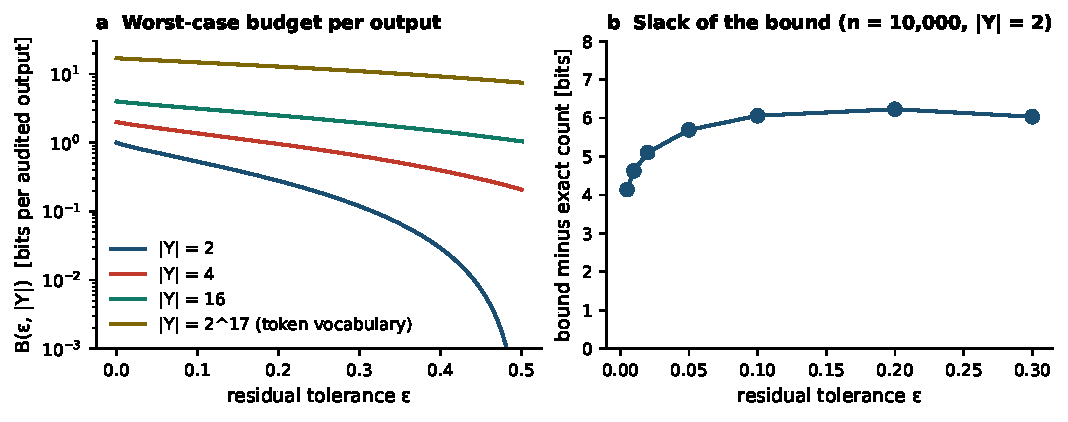
\includegraphics[width=\textwidth]{figures/fig_budget.pdf}
\caption{\textbf{The worst-case explanation budget per audited output.} \textbf{a}, $B(\varepsilon,q)$ of Theorem~\ref{thm:counting}: the number of bits of explanation that every audited output costs, in the worst case over behaviours, as a function of the residual tolerance $\varepsilon$ and the output alphabet size $q=|\Y|$. It is positive for every $q\ge2$ and $\varepsilon<\frac12$. \textbf{b}, Slack of the entropy bound against the exact Hamming-ball count for $n=10{,}000$ binary decisions at seven tolerances: the bound used in the theorem is loose by 4.1 to 6.2 bits out of $10^{4}$.}
\label{fig:budget}
\end{figure}

\subsection{The optimal explanation score is uncomputable}

For this result let $\X=\{x_1,x_2,\dots\}$ be countably infinite with a fixed computable enumeration, and for a table $t\in\Y^{n}$, $n\ge1$, let $\D_t:=((x_1,t_1),\dots,(x_n,t_n))$ and $L^{*}(t):=\inf_{E\in\LU}L_{\D_t}(E)$ be the minimal two-part code length over the universal language.

\begin{theorem}[uncomputability]
\label{thm:uncomputable}
No algorithm, given $t\in\Y^{*}$, outputs a number within $\frac12$ of $L^{*}(t)$; the same holds for any fixed additive precision. Consequently the optimal explanation compression score $\ECS^{*}(t)=1-L^{*}(t)/(n\Ltwo q)$ is not computable to within $1/(2n\Ltwo q)$, and in particular not exactly.
\end{theorem}

\begin{corollary}[a checkable standard fixes the language]
\label{cor:checkable}
A requirement phrased as ``provide the best, complete, or optimal explanation'' over an unrestricted language is not effectively checkable. A checkable requirement specifies a decidable explanation language $\Lang$ with computable semantics, the residual metric, thresholds $(\ell_{\max},\varepsilon)$ and the audit distribution, and is existential: ``exhibit an explanation meeting $(\ell_{\max},\varepsilon)$''. Scores are comparable across models only within the same $\Lang$.
\end{corollary}

The theorem is a corollary of the classical fact that no unbounded computable function is a lower bound for Kolmogorov complexity \citep[\S2.3]{livitanyi2008}, and uncomputability of MDL-optimal two-part codes is itself classical \citep{vereshchagin2004}. What is new is the reading for standards. For a finite or decidable language with total computable semantics, such as attribution graphs with at most $k$ nodes over a fixed feature dictionary, the $\Lang$-optimum is computable by exhaustive search, merely exponential in the budget; a graph returned by pruning \citep{ameisen2025circuit} is then an upper bound on the $\Lang$-optimal length at its observed residual, which is exactly what an existential standard asks for. The EU AI Act and the EASA framework both use the word ``explainability'' without fixing a language \citep{euaiact2024,easa2024}; Corollary~\ref{cor:checkable} says what their harmonised standards must add for the requirement to be auditable.

\subsection{Faithfulness and correctness are independent}

Let $g:\X\to\Y$ be the ground truth for the task, $M$ deterministic, and $\err_{\D}(M):=\frac1n\sum_i\ind{M(x_i)\neq g(x_i)}$.

\begin{theorem}[independence]
\label{thm:independence}
(i) Fix any model $M$, explanation $E$ and audit set $\D$ of $n$ distinct inputs, so that $\ell(E)$, $R_{\D}(E)$ and $\ECS_{\D}(E)$ are all fixed. For every $b\in\{0,\frac1n,\dots,1\}$ there is a ground truth $g$ with $\err_{\D}(M)=b$. (ii) Conversely, for every $g$ taking at least two values and every $v\in[0,1]$ there are an audit multiset $\D$, a model $M$ with $\err_{\D}(M)=0$, and an explanation $E$ of constant length with $R_{\D}(E)=v$ up to the grid $\frac1n$.
\end{theorem}

\begin{corollary}[certification has two channels]
\label{cor:twochannel}
No function of $(\ell(E),R_{\D}(E),\ECS_{\D}(E),M,\D)$ bounds $\err_{\D}(M)$ below 1. A sound certification combines a \emph{faithfulness channel}, which is what an explanation score measures, with an independent \emph{correctness channel}: labels, a specification, a formal check, or human review of a sample (Figure~\ref{fig:channels}).
\end{corollary}

Theorem~\ref{thm:independence} is immediate; we state it because its regulatory consequence is not. It is the formal version of the distinction between faithfulness and plausibility \citep{jacovi2020,lipton2018}, and it applies equally to models that are interpretable by construction \citep{rudin2019}: a transparent mechanism is still a statement about the mechanism. An auditor who sees the model, the explanation and the outputs, but no ground truth, has no information about whether the outputs are right: explanation quality is a statement about the model's mechanism, correctness is a statement about the world. What a residual can legitimately signal is anomaly. If a reference explanation $E^{*}$ is $\varepsilon$-faithful on a trusted input distribution, a large $r_{E^{*}}(x)$ on a new input says that the model produced its output by a mechanism $E^{*}$ does not cover; this is the mechanistic anomaly detection programme of \citet{christiano2022mad} and \citet{jenner2024mad}. Whether mechanism anomalies correlate with errors on a given task is an empirical fact about that task and model, which is why the experiment of Section~\ref{sec:experiment} exists.

\begin{figure}[t]
\centering
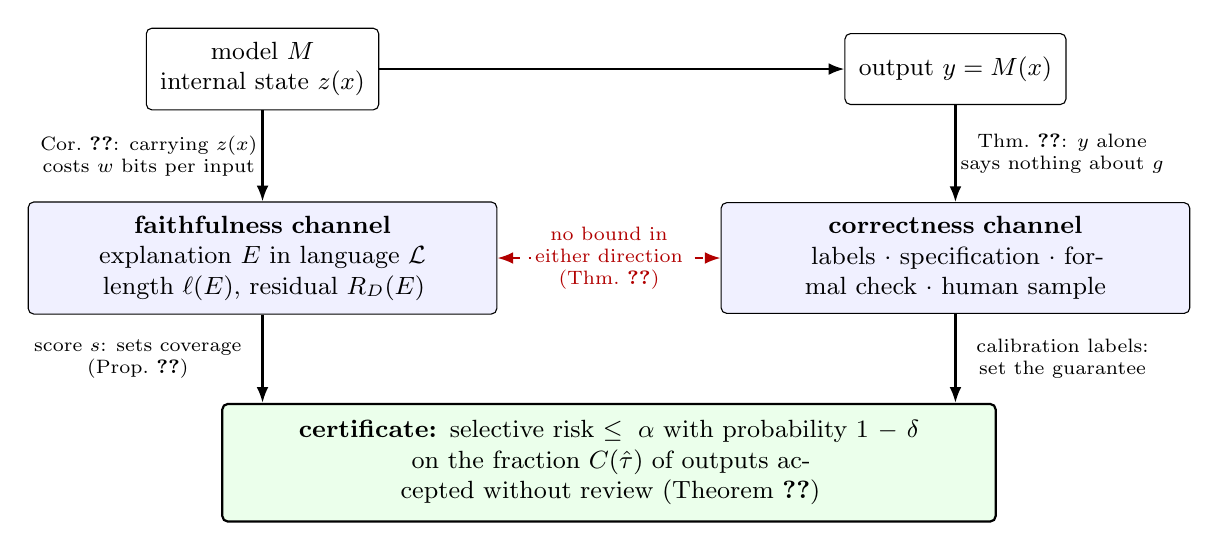
\begin{tikzpicture}[x=1cm,y=1cm,
  box/.style={draw,rounded corners=2pt,align=center,minimum height=9mm,inner sep=5pt,font=\small},
  chan/.style={draw,rounded corners=2pt,align=center,minimum height=9mm,inner sep=5pt,font=\small,fill=blue!6,text width=5.6cm},
  cert/.style={draw,thick,rounded corners=2pt,align=center,minimum height=11mm,inner sep=6pt,font=\small,fill=green!8,text width=9.4cm},
  arr/.style={-{Latex[length=2mm]},thick},
  lab/.style={font=\scriptsize,align=center,fill=white,inner sep=1.5pt}
]
\node[box] (model) at (0,0) {model $M$\\ internal state $z(x)$};
\node[box] (out) at (8.8,0) {output $y=M(x)$};
\draw[arr] (model) -- (out);
\node[chan] (expl) at (0,-2.4) {\textbf{faithfulness channel}\\ explanation $E$ in language $\Lang$\\ length $\ell(E)$, residual $R_{\D}(E)$};
\node[chan] (truth) at (8.8,-2.4) {\textbf{correctness channel}\\ labels $\cdot$ specification $\cdot$ formal check $\cdot$ human sample};
\node[cert] (cert) at (4.4,-5.0) {\textbf{certificate:} selective risk $\le\alpha$ with probability $1-\delta$\\ on the fraction $C(\tauhat)$ of outputs accepted without review (Theorem~\ref{thm:selective})};
\draw[arr] (model) -- node[lab,left] {Cor.~\ref{cor:state}: carrying $z(x)$\\ costs $w$ bits per input} (expl);
\draw[arr] (out) -- node[lab,right] {Thm.~\ref{thm:independence}: $y$ alone\\ says nothing about $g$} (truth);
\draw[arr] (expl.south) -- node[lab,left,xshift=-2mm] {score $s$: sets coverage\\ (Prop.~\ref{prop:value})} (cert.north -| expl.south);
\draw[arr] (truth.south) -- node[lab,right,xshift=2mm] {calibration labels:\\ set the guarantee} (cert.north -| truth.south);
\draw[{Latex[length=2mm]}-{Latex[length=2mm]},thick,red!70!black,dashed] (expl.east) -- node[lab,text=red!70!black] {no bound in\\ either direction\\ (Thm.~\ref{thm:independence})} (truth.west);
\end{tikzpicture}
\caption{\textbf{Certification has two channels.} The explanation channel measures how faithfully a short description reproduces the model's behaviour; the correctness channel measures whether the behaviour is right. Theorem~\ref{thm:independence} says that neither bounds the other. In the certified selective deployment of Theorem~\ref{thm:selective}, the correctness channel sets the guarantee and the explanation, used as a score, sets only the fraction of outputs that can be accepted without review.}
\label{fig:channels}
\end{figure}

\subsection{Chain of thought under the score}

A chain of thought $c(x)$ states reasons and an answer $a(x)$. Read it as the explanation $E_c$: ``given these stated reasons, the answer is $a(x)$''. Under the side-information rule its length is the bits of the text, typically $10^{3}$ to $10^{4}$ per input, and that length is paid per input, because nothing in a transcript is amortised across inputs.

\begin{proposition}[chain of thought]
\label{prop:cot}
(i) \emph{Negative gain.} For any per-input textual explanation with average length $\bar w$ bits per input, $G_{\D}(E_c)\le n(\Ltwo q-\cz-\bar w)$, which is negative whenever $\bar w>\Ltwo q-\cz$, that is, above about 17 bits per output for a vocabulary of $2^{17}$. (ii) \emph{Interventional residual.} Let $\D'$ consist of pairs $(u_i,M(u_i))$, $i=1,\dots,n'$, where each $u_i$ is obtained from $x_i$ by an intervention that preserves every reason $c(x_i)$ states and alters an unstated factor, when such an intervention is available; where it is not, because every candidate factor is stated, take $u_i:=x_i$, the trivial intervention, so that $M(u_i)=a(x_i)$. Define $r_c(x_i):=\ind{M(u_i)\neq a(x_i)}$, which is 0 under the trivial intervention. If the stated reasons are the complete causes of the answer then $r_c\equiv0$; if $r_c=1$ on a fraction $\varphi$ of $\D'$, the correction term of $E_c$ on $\D'$ is $\varphi n'\co+(1-\varphi)n'\cz$.
\end{proposition}

The design of \citet{chen2025reasoning} realises $\D'$ with an inserted hint as the unstated factor. Take $\D'$ to be the inputs on which the hint changed the model's answer. For those whose chain of thought does not mention the hint, removing it preserves every stated reason and restores the unhinted answer, so $r_c=1$; for those that state the hint, the intervention is trivial and $r_c=0$. The measured rates of mentioning a used hint, 25\% and 39\% averaged across six hint types for the two reasoning models studied, therefore put $\varphi$ at 61 to 75\%. In the same study, models trained in environments with exploitable reward signals learned to exploit them and in most cases did not say so in their chains of thought, and outcome-based training raised faithfulness only briefly before plateauing; earlier work found the same unfaithfulness in non-reasoning models \citep{turpin2023}; an empirical study of training against chain-of-thought monitors found that the pressure teaches models to hide their intent \citep{baker2025monitoring}; and a multi-laboratory position paper warns that whatever monitorability exists is fragile to training choices \citep{korbak2025}. Proposition~\ref{prop:cot} places the chain of thought precisely: it is a legible monitor for frequent, multi-step misbehaviour, which is where \citet{chen2025reasoning} also place it; it is not a certificate. The only way a textual explanation can score positively in this framework is to be amortised, a rule stated once that predicts outputs across many inputs. That is a circuit, not a transcript.

\section{What can be certified}
\label{sec:certify}

\subsection{Certified selective deployment}

Let $P$ be a distribution on pairs $(X,G)$ of inputs and ground-truth labels, let $M$ be deterministic, and let $\lambda(x,g):=\ind{M(x)\neq g}$ be the 0-1 loss. A \emph{score} is any function $s:\X\to\R$ of the input and the model's internals, for example the residual $r_{E^{*}}(x)$ of a reference explanation, the error-node mass of an attribution graph, or the model's own confidence; $s$ and $M$ are fixed before the calibration sample is drawn. The policy $\pi_\tau$ accepts an output when $s(x)\le\tau$ and defers it to a human otherwise. Coverage is $C(\tau):=P(s(X)\le\tau)$ and selective risk is $R(\tau):=P(M(X)\neq G\mid s(X)\le\tau)$, defined when $C(\tau)>0$.

Draw $m$ calibration pairs $(x_j,g_j)$ i.i.d.\ from $P$, with labels from the correctness channel, and fix a grid $\tau_1<\dots<\tau_K$ independently of the sample. For each $k$ let $A_k:=\{j:s(x_j)\le\tau_k\}$, $m_k:=|A_k|$, $e_k:=\sum_{j\in A_k}\lambda(x_j,g_j)$, and let $\UCB_k$ be the one-sided Clopper--Pearson upper bound \citep{clopper1934} at level $1-\delta/K$ for a binomial proportion with $m_k$ trials and $e_k$ successes ($\UCB_k:=1$ when $m_k=0$):
\begin{equation}
\UCB_k:=\sup\Big\{p\in[0,1]:\ \Pr_{\Bin(m_k,p)}\big[S\le e_k\big]\ge\delta/K\Big\}.
\end{equation}
Set $\tauhat:=\max\{\tau_k:\UCB_k\le\alpha\}$, and write $\tauhat=\bot$ (defer everything) if no $k$ qualifies.

\begin{theorem}[certified selective deployment]
\label{thm:selective}
For every score $s$ and model $M$ fixed independently of the calibration sample, every $\alpha,\delta\in(0,1)$, and every grid fixed independently of it, if the calibration pairs are i.i.d.\ from the deployment distribution $P$ then
\begin{equation}
\Pr\big[\,R(\tauhat)\le\alpha\ \text{ or }\ \tauhat=\bot\,\big]\ \ge\ 1-\delta,
\end{equation}
the probability being over the calibration sample.
\end{theorem}

The theorem is the selective classification guarantee of \citet{geifman2017} in the form of a fixed-grid Learn-then-Test procedure \citep{angelopoulos2021ltt,bates2021rcps}, with the reject option going back to \citet{chow1957,chow1970}, the finite-sample theory to \citet{elyaniv2010,vovk2005}, and the deferral policy itself studied as learning to defer \citep{madras2018,mozannar2020}. Tighter valid procedures exist: fixed-sequence testing, valid for any pre-specified order and tight when the risk is monotone in $\tau$, conformal risk control \citep{angelopoulos2022crc}, selective conformal risk control \citep{xu2025scrc}, and betting-based confidence sequences \citep{basu2026}. We state the simplest valid version because our interest is in what it does not depend on.

\paragraph{What the theorem does not promise.} The guarantee is marginal over inputs; subgroups can carry higher risk, and the grouping-loss estimators of \citet{melo2026} address this. It needs i.i.d.\ sampling from the deployment distribution with the score, the model and the grid fixed in advance: distribution shift, adversarial inputs, feedback loops, a score tuned on the calibration data, and a grid taken from the sample's own quantiles all void it, and Section~\ref{sec:simulation} shows the per-threshold statement behind the proof failing for the last of these. It bounds error as the calibration labels define it. And the deferred channel has its own error: total error is at most $C(\tauhat)\alpha+(1-C(\tauhat))\rho_h$, where $\rho_h$ is the reviewer's miss rate.

\paragraph{The point on which the rest turns.} Theorem~\ref{thm:selective} holds for a random score. The guarantee never depends on the score; only the coverage $C(\tauhat)$ does. In this certificate, interpretability enters, if at all, through the score, and its value there is the coverage it adds. It can in principle also serve the correctness channel, through formal proofs of performance bounds extracted from mechanistic understanding \citep{gross2024}; that route has so far been demonstrated on toy models, and its obstacle, compounding structureless error, is the residual of Definition~\ref{def:residual} under another name.

\subsection{The value of a score}

Let $c_h$ be the cost of one human review, $c_s$ the marginal cost of computing score $s$ per request, and $C_s(\alpha)$ the coverage that Theorem~\ref{thm:selective} certifies with score $s$ at risk $\alpha$ (a random quantity, through the calibration sample).

\begin{proposition}[value identity]
\label{prop:value}
Over $N$ requests, the saving from using score $s$ instead of a baseline $s_0$, both calibrated to the same $(\alpha,\delta)$ on the same sample, is
$\Delta=N\big[(C_s(\alpha)-C_{s_0}(\alpha))\,c_h-(c_s-c_{s_0})\big]$,
so $s$ is worth adopting if and only if $(C_s(\alpha)-C_{s_0}(\alpha))\,c_h>c_s-c_{s_0}$.
\end{proposition}

The identity is bookkeeping, but it is the sentence a deployer will ask a vendor to prove. A compliance analyst spending one to fifteen minutes per output at a loaded rate of 120 to 200 dollars an hour gives $c_h$ of about 2 to 50 dollars. An attribution graph on a two-billion-parameter model costs tens of replacement-model forward passes plus attribution, roughly 10 to 100 plain forward passes, more on a frontier model; at $10^{-4}$ to $10^{-2}$ dollars per forward pass, from a small open model on owned hardware to a frontier model behind an API, $c_s$ is about 0.001 to 1 dollar. The break-even coverage gain $\Delta c_s/c_h$ is therefore anywhere from 0.002 to 50 percentage points. That range is the point: the decision is made by measuring $\Delta C$, not by argument.

\subsection{Regress and the trusted base}

If the labels used to calibrate come from a checker $V$ that can itself be wrong, the certified bound loosens by that checker's miss rate, and a chain of checkers loosens it by every learned link in the chain.

\begin{proposition}[regress]
\label{prop:regress}
Let the calibration labels be produced by a checker $V$ whose verdict is a fixed function of $(x,M(x))$, let $R_V(\tau):=\Pr[V\text{ says wrong}\mid s(X)\le\tau]$ be the risk Theorem~\ref{thm:selective} controls with $V$'s labels, and let $\rho_V:=\Pr[M(X)\neq G\text{ and }V\text{ says correct}\mid s(X)\le\tauhat]$ be $V$'s conditional miss rate on accepted outputs. On the event of Theorem~\ref{thm:selective},
$R(\tauhat)\le R_V(\tauhat)+\rho_V\le\alpha+\rho_V$.
If a second checker $V_2$ audits a random sample of $N_2$ accepted outputs that $V$ passed, then with probability at least $1-\delta_2$, $\rho_V\le\hat\rho_{12}+\varepsilon_2(N_2,\delta_2)+\rho'_{V_2}$, where $\hat\rho_{12}$ is the rate at which $V_2$ overturns $V$ on that sample, $\varepsilon_2$ is the one-sided binomial slack and $\rho'_{V_2}$ is $V_2$'s own conditional miss rate on it.
\end{proposition}

The chain is useful only if its last term is bounded by means outside the learned stack: a formal proof, an exhaustive test, or a human audit whose own miss rate is estimated from a random sample. Call the set of such terminal checkers the \emph{trusted base} of a certification. The trusted base can be small, which is the practical content of the observation that a checker can confirm primality without understanding primes, but it cannot be empty, and every learned link adds a term the chain itself cannot see. The analogy with G\"odel's second theorem \citep{godel1931}, that a system expressive enough to reason about its own correctness cannot establish it, is only an analogy: Proposition~\ref{prop:regress} is a union bound, not an incompleteness phenomenon. What it shares with the theorem is the conclusion that self-certification does not close.

\section{Simulation study}
\label{sec:simulation}

We validate Theorem~\ref{thm:selective} on synthetic deployment distributions whose risk curves are known exactly, in closed form or from the bivariate normal distribution function, so that the true selective risk of every chosen threshold is known, and we test which hypotheses can be dropped. Protocols are in Methods; code and seeds are in the companion repository.

\paragraph{The certified risk is controlled, conservatively.} With scores $s\sim\Unif(0,1)$, error probability $0.0025+0.6s^{2}$, a fixed grid of $K=50$ thresholds, $\delta=0.05$ and $10^{4}$ replications per setting, the frequency with which the certified threshold's true risk exceeded $\alpha$ was at most $5\times10^{-4}$ for $\alpha=0.05$ and at most $4\times10^{-4}$ for $\alpha=0.01$, two orders of magnitude below the nominal $\delta$ (Table~\ref{tab:violation}; at this resolution a rate of $10^{-4}$ is one event in $10^{4}$, with a 95\% interval of 0 to $5.6\times10^{-4}$). The slack is the price of the union bound and of the discreteness of the exact binomial bound; tighter valid procedures recover much of it once the calibration set is large enough to make their tests powerful \citep{angelopoulos2021ltt,basu2026}; the fixed-sequence variant in the companion code, for instance, defers everything at small $m$ under an ascending order and overtakes the Bonferroni procedure's coverage only at $m=8{,}000$. The guarantee is a statement about the procedure, not about a lucky calibration: it holds unconditionally only because deferring everything counts as success. Conditional on the rare event of not deferring at a small sample size, the chosen threshold is selected for luck, and its conditional violation rate is high (3 of 3 non-deferred replications at $m=250$, $\alpha=0.05$). A deployer who observes a non-deferral at small $m$ cannot read the certificate as a conditional guarantee.

\begin{table}[t]
\centering\small
\caption{\textbf{Frequency with which the certified threshold's true selective risk exceeds $\alpha$}, over $10^{4}$ calibration draws per cell, with the fraction of draws in which the procedure deferred everything in parentheses; deferring everything counts as success. Nominal bound $\delta=0.05$. The valid procedure is two orders of magnitude inside its bound. The sample-quantile grid does not raise the end-to-end rate here but invalidates the per-threshold statement on which the proof rests (text). Omitting the multiplicity correction raises the rate to as much as 3.1\% (0.8\% to 2.9\% at $\alpha=0.05$; up to 3.1\% at $\alpha=0.01$ once the procedure stops deferring everything), still under $\delta$ in this setting because the $K$ nested tests are positively dependent, but with no guarantee.}
\label{tab:violation}
\setlength{\tabcolsep}{3.5pt}\footnotesize
\begin{tabular}{rcccccc}
\toprule
 & \multicolumn{2}{c}{Theorem~\ref{thm:selective}} & \multicolumn{2}{c}{sample-quantile grid} & \multicolumn{2}{c}{no multiplicity correction} \\
\cmidrule(lr){2-3}\cmidrule(lr){4-5}\cmidrule(lr){6-7}
$m$ & $\alpha=0.01$ & $\alpha=0.05$ & $\alpha=0.01$ & $\alpha=0.05$ & $\alpha=0.01$ & $\alpha=0.05$ \\
\midrule
250 & $<\!10^{-4}$ (100\%) & 0.0003 (100\%) & $<\!10^{-4}$ (100\%) & 0.0004 (100\%) & $<\!10^{-4}$ (100\%) & 0.0292 (56\%) \\
500 & $<\!10^{-4}$ (100\%) & 0.0005 (91\%) & $<\!10^{-4}$ (100\%) & 0.0004 (91\%) & $<\!10^{-4}$ (100\%) & 0.0262 (12\%) \\
1000 & $<\!10^{-4}$ (100\%) & 0.0005 (35\%) & $<\!10^{-4}$ (100\%) & 0.0006 (33\%) & 0.0016 (100\%) & 0.0236 (0\%) \\
2000 & $<\!10^{-4}$ (100\%) & 0.0001 (1\%) & $<\!10^{-4}$ (100\%) & 0.0001 (1\%) & 0.0181 (91\%) & 0.0195 (0\%) \\
4000 & $<\!10^{-4}$ (100\%) & 0.0001 (0\%) & 0.0001 (100\%) & 0.0002 (0\%) & 0.0310 (62\%) & 0.0148 (0\%) \\
8000 & 0.0004 (95\%) & $<\!10^{-4}$ (0\%) & 0.0001 (94\%) & 0.0002 (0\%) & 0.0236 (29\%) & 0.0080 (0\%) \\
\bottomrule
\end{tabular}

\end{table}

\paragraph{Coverage approaches the oracle as the sample grows.} At $\alpha=0.05$ the certified policy accepted 18\% of outputs with $m=1{,}000$ calibration points, 33\% with $2{,}000$ and 42\% with $8{,}000$, against an oracle of 48\% (Figure~\ref{fig:sim}a). Certifying $\alpha=0.01$ on the same distribution required far more data: the procedure deferred everything in at least 94\% of replications up to $m=8{,}000$, against an oracle coverage of 18\%. A one-percent certified risk needs a calibration set an order of magnitude larger than a five-percent one.

\paragraph{Dropping a hypothesis.} Replacing the fixed grid by the calibration sample's own quantiles did not raise the end-to-end violation rate here (at most $6\times10^{-4}$), but it falsifies the per-threshold statement from which Theorem~\ref{thm:selective} is proved. With $m=50$ uniform scores, error probability $\ind{s<0.3}$ and the threshold taken as the 20th order statistic, the true risk at the chosen threshold exceeded its nominal 95\% upper bound in 6.17\% of $2\times10^{6}$ replications, against 3.00\% for the fixed threshold at that order statistic's expectation. A practitioner who reports ``the risk at my threshold is below this bound with 95\% confidence'' after choosing the threshold from the data is reporting something false.

\paragraph{Score quality buys coverage, not validity.} With a latent error signal $z\sim N(0,1)$, errors when $z$ exceeds its 90th percentile, and scores $s=z+\sigma\xi$ of decreasing quality, the violation rate stayed at or below $10^{-3}$ for every score while certified coverage at $\alpha=0.05$ and $m=2{,}000$ rose from 1\% at AUROC $0.67$ (96\% of replications deferred everything) through 26\% at $0.74$, 55\% at $0.80$, 75\% at $0.88$ and 83\% at $0.92$ to 92\% at $0.99$, against oracle coverages of 39\% to 94\% (Figure~\ref{fig:sim}b). Raising a score's AUROC from 0.80 to 0.92 raised certified coverage by 29 percentage points; by Proposition~\ref{prop:value} that is worth $0.29\,c_h$ per request, about 1.45 dollars at $c_h=5$ dollars, before the score's own cost. This is the quantity the experiment of Section~\ref{sec:experiment} measures for explanation residuals.

\begin{figure}[t]
\centering
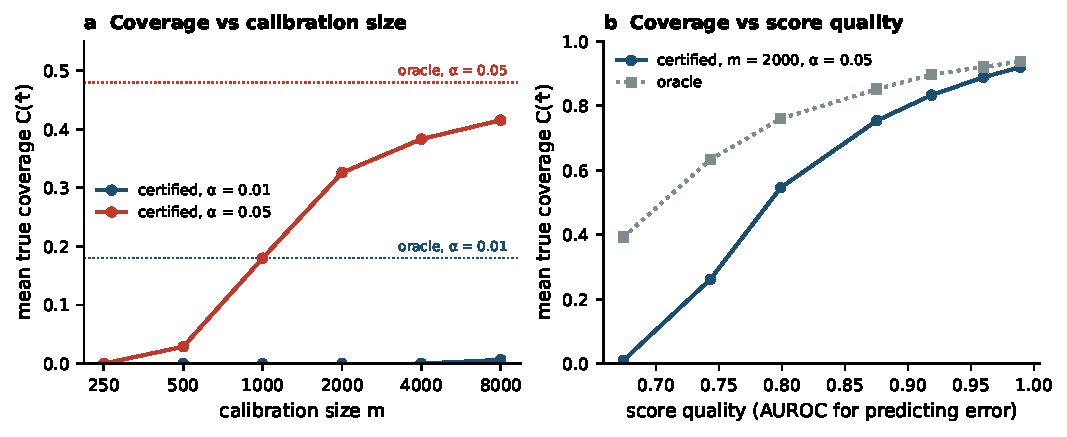
\includegraphics[width=\textwidth]{figures/fig_simulation.pdf}
\caption{\textbf{Certified coverage in simulation.} \textbf{a}, Mean true coverage $C(\tauhat)$ of the certified threshold of Theorem~\ref{thm:selective} against calibration size, at $\alpha\in\{0.01,0.05\}$ and $\delta=0.05$, with the oracle coverage (the largest grid threshold whose true risk is at most $\alpha$) as dotted lines; $10^{4}$ calibration draws per point. \textbf{b}, Certified coverage at $\alpha=\delta=0.05$ and $m=2{,}000$ as a function of the score's AUROC for predicting error, with the oracle coverage; $2{,}000$ calibration draws per point. The violation rate was at or below $10^{-3}$ at every point of both panels (Table~\ref{tab:violation} and text). Validity is unchanged across scores; coverage is what a better score buys.}
\label{fig:sim}
\end{figure}

\section{Instantiation: attribution graphs under the accounting}
\label{sec:instantiation}

Attribution graphs \citep{ameisen2025circuit,lindsey2025biology} are the most developed candidate for an explanation language, and the accounting of Section~\ref{sec:setting} sorts their components into what is an explanation and what is a second model.

An attribution graph for a prompt $x$ is computed from a \emph{replacement model} in which the model's MLP layers are replaced by a cross-layer transcoder dictionary $\mathcal{D}_T$ trained on the model's own activations \citep{bricken2023,lieberum2024gemmascope}, while the attention patterns and normalisation denominators are taken from the underlying model's forward pass on $x$ \citep{ameisen2025circuit}. The graph's nodes are active dictionary features, token embeddings, output logits and \emph{error nodes}, the last carrying the part of each MLP output that the dictionary does not reconstruct; its edges are linear effects between nodes. Pruned to $k$ feature nodes and $k'$ edges with weights quantised to $p$ bits, the graph itself has length $k\Ltwo|\mathcal{D}_T|+k'(p+2\lceil\Ltwo k\rceil)+O(\log k)$ bits, several kilobits. Under the side-information rule two further charges apply. The dictionary is trained on the model and is therefore model-specific: its description, of order $10^{10}$ bits for a two-billion-parameter model, is charged to the audit set and amortised over its $n$ prompts, which is $10^{6}$ to $10^{7}$ bits per prompt for audits of $10^{3}$ to $10^{4}$. The frozen attention patterns are functions of the model's state on the prompt, at least $10^{5}$ bits per prompt for a model with 26 layers and 8 heads even on prompts of tens of tokens, and are charged per prompt. Both charges exceed the 17 or 18 bits that an output is worth by roughly four to six orders of magnitude.

The conclusion is not that the graphs are useless but that, as per-prompt objects, they are not explanations in the sense of Definition~\ref{def:ecs}: a replacement model that reproduced the model exactly would be a second model, to which Theorem~\ref{thm:selfref} applies as to the first; one that reproduces it only approximately pays Lemma~\ref{lem:identity}'s charge for every disagreement; and in either case its frozen per-prompt state falls under Corollary~\ref{cor:state}. How the graphs are used in practice is consistent with this. Across many prompts they are used to find short rules, for example the parallel heuristics by which a model adds two-digit numbers \citep{lindsey2025biology}; a rule of that kind, stated once, applied to the whole audit set, and evaluated by semantics that do not call the model, is an explanation whose length and residual Definition~\ref{def:ecs} measures. And per prompt, a graph supplies scores for Theorem~\ref{thm:selective}, in decreasing order of faithfulness and cost: the total-variation distance between the model and the replacement model run with only the graph's features active and its error nodes zeroed; the \emph{error-node mass}, the share of attribution to the target logit that flows from the error nodes; and the dictionary's reconstruction error at the final layers, which costs one forward pass.

Where the residual stands today is documented by the method's authors. The replacement model built from cross-layer transcoders matches the underlying model's output in about half of cases \citep{ameisen2025circuit}; the graphs are faithful only with their error nodes included, and the error nodes are unexplained by construction. A 2026 study of jailbreaks with attribution graphs reports that including the error nodes reduced the KL divergence between the attribution model and the underlying model by 99.997\%, from 46.96 to 0.0014, on its sample of ten prompts \citep{wagle2026jailbreak}. Sparse-dictionary reconstruction error follows a power law with a persistent floor, and the error is itself largely predictable from the activations \citep{engels2024darkmatter,gao2024scaling}. Read through Definition~\ref{def:ecs}, the pruned graph without its error nodes carries a large correction term on many prompts, as Theorem~\ref{thm:counting} predicts for any budget below the behaviour's complexity. Automated annotation of graphs \citep{patel2026annotate} lowers the labelling cost but not the residual. A recent position paper in computer vision asks that the understandability of models be measured with independent evaluators rather than inferred from methods \citep{colin2026}; Definition~\ref{def:ecs} is a model-centric measure of a different kind, of compression rather than of human understanding. The graph's value for certification is the empirical one that Section~\ref{sec:experiment} measures: whether its residuals predict error better than the model's own confidence.

\section{Implications for regulation and standards}
\label{sec:regulation}

\paragraph{Explanations can be required; their existence cannot.} Corollary~\ref{cor:defer} says that any standard of the form ``accept only what is explained within a fixed budget'' must contain a defer outcome, and Corollary~\ref{cor:permodel} says which behaviours land there: those more complex than the budget. Human oversight of the deferred class is therefore a mathematical consequence of fixing a budget, not only a policy choice. Article~14 of the AI Act, read in this light, is the law requiring what the counting argument requires anyway.

\paragraph{A requirement to explain must name the language.} Corollary~\ref{cor:checkable} gives the harmonised standards being drafted under the Act, and the explainability provisions of the EASA framework \citep{easa2024} and the ED-324/ARP6983 process standard \citep{ed324}, a concrete test of auditability: the standard must specify the explanation language, the residual metric, the thresholds and the audit distribution, and must be existential rather than optimal. A requirement that fails this test cannot be checked effectively by anyone, including the regulator.

\paragraph{Explanation does not discharge the duty to validate.} Theorem~\ref{thm:independence} means that no explanation, however faithful, can stand in for outcomes analysis or a specification. For model-risk management under SR~11-7 \citep{sr117}, interpretability belongs to conceptual soundness, not to outcomes analysis, and cannot be traded against it.

\paragraph{What can be certified today.} Theorem~\ref{thm:selective} gives a regulated deployer a certificate of the form ``with probability at least $1-\delta$ over the calibration draw, the error rate among auto-accepted outputs is at most $\alpha$'', using whatever score the deployer already has and labels its reviewers already produce. The policy keeps human oversight for the deferred class, so it reduces review rather than claiming to abolish it. The certificate's hypotheses, i.i.d.\ sampling with the score, model and grid fixed in advance, translate into operational requirements: a fixed audit protocol, recalibration on fresh labelled samples, and monitoring for shift. The deferred deadlines for high-risk obligations under the Act, 2 December 2027 for standalone systems and 2 August 2028 for product-embedded ones \citep{euomnibus2026}, are the horizon on which such certificates will be asked for.

\paragraph{The role left for interpretability.} Within the certificate of Theorem~\ref{thm:selective} it is the score. An explanation residual that predicts error better than the model's own confidence raises certified coverage and lowers review cost by exactly Proposition~\ref{prop:value}; one that does not is a cost. The question is empirical and narrow, and it is the subject of the next section.

\section{Limitations and a pre-registered experiment}
\label{sec:experiment}

Theorems~\ref{thm:selfref}--\ref{thm:independence} are worst-case or structural statements; none says that a particular trained model is unexplainable on a particular audit set, and Theorem~\ref{thm:uncomputable} is specific to the universal language. Theorem~\ref{thm:selective} is marginal, needs i.i.d.\ sampling, and inherits the noise of its labels (Proposition~\ref{prop:regress}). The simulations use synthetic distributions chosen for exact ground truth, not real models.

The one question this paper leaves open is whether an explanation residual predicts a model's errors well enough to raise certified coverage over cheap uncertainty scores at a compute cost below the review cost it saves. We pre-register the experiment that tests it (Appendix~\ref{app:prereg}): Gemma-2-2B and Llama-3.2-1B with open transcoders and the open circuit-tracing library; three tasks with deterministic ground truth (factual recall, two-digit addition, a four-way MMLU subset) and a fourth, hint-injection condition that changes the mechanism without changing the task; three explanation residuals (error-node mass, replacement-model total variation, final-layer reconstruction error) against five baselines (maximum softmax probability, predictive entropy, self-consistency disagreement, verbalised confidence, and the epistemic-risk estimator of \citet{melo2026}); AUROC with DeLong intervals and certified coverage at $\alpha\in\{1\%,5\%\}$ under Theorem~\ref{thm:selective}, with the 1\% condition expected to defer everything unless a task's error rate is far below 1\%. Our prior, written before any data: a 30 to 45\% probability that some residual beats the best baseline in distribution on at least one task, 25 to 40\% that it raises certified coverage there, and 50 to 65\% that some residual beats every baseline under the hint condition, where the residual is defined against trusted-data mechanisms and a hint is a mechanism change that confidence does not see. Either outcome is reported: a positive result would be evidence that an explanation residual has certification value in the role the theory leaves it short of a formal proof; a negative one would show, for these models and tasks, that it does not, leaving Theorem~\ref{thm:selective} with existing scores as the available offer.

\section*{Methods}

\paragraph{Formal conventions.} All results use the definitions of Section~\ref{sec:setting}. Full proofs are in Appendix~\ref{app:proofs}. The one-sided Clopper--Pearson bound and its coverage property are stated and proved as Lemma~\ref{lem:cp}.

\paragraph{Simulation A (validity and coverage).} Scores $s_j\sim\Unif(0,1)$ and errors $\lambda_j\sim\mathrm{Bernoulli}(0.0025+0.6s_j^{2})$, independently, so that $R(\tau)=0.0025+0.2\tau^{2}$ and $C(\tau)=\tau$ in closed form; the constant $0.0025$ keeps every grid point off the boundaries $R=0.01$ and $R=0.05$. Grid $\tau_k=k/50$, $k=1,\dots,50$, fixed. For each $m\in\{250,500,1000,2000,4000,8000\}$, $10^{4}$ independent calibration samples; for each, the Bonferroni threshold of Theorem~\ref{thm:selective} at $\delta=0.05$ and $\alpha\in\{0.01,0.05\}$, the same with Clopper--Pearson at level $1-\delta$ and no multiplicity correction, and the same with the grid replaced by the sample's own $k/50$ quantiles. Reported: the frequency, over all replications, of a non-deferred $\tauhat$ with $R(\tauhat)>\alpha$ (so that deferring everything counts as success, as in the statement of Theorem~\ref{thm:selective}), the frequency of deferring everything, and the mean of $C(\tauhat)$ with $C(\bot):=0$; the oracle is the largest grid point with $R(\tau_k)\le\alpha$.

\paragraph{Simulation B (per-threshold statement).} $m=50$ scores $\sim\Unif(0,1)$, error indicator $\ind{s<0.3}$, so that $R(\tau)=\min(1,0.3/\tau)$. Threshold $\tau$ either the 20th order statistic of the scores or the fixed value $20/51$; $\UCB$ the 95\% one-sided Clopper--Pearson bound on the accepted set; $2\times10^{6}$ replications; reported is the frequency of $R(\tau)>\UCB$.

\paragraph{Simulation C (score quality).} Latent $z\sim N(0,1)$; error when $z>\Phi^{-1}(0.9)$; score $s=z+\sigma\xi$ with $\xi\sim N(0,1)$ and $\sigma\in\{0.25,0.5,0.75,1,1.5,2,3\}$. On a fixed grid of 60 points on $[-3,3]$, $C(\tau_k)=\Phi(\tau_k/\sqrt{1+\sigma^{2}})$ and $R(\tau_k)$ in closed form from the bivariate normal distribution of $(z,s)$, which has correlation $1/\sqrt{1+\sigma^{2}}$; the AUROC label of each score is estimated by $4\times10^{5}$ paired Monte Carlo draws. $2{,}000$ calibration samples of size $m=2{,}000$ per $\sigma$; Bonferroni threshold at $\alpha=\delta=0.05$; reported as in Simulation A.

\paragraph{Software.} Python 3 with NumPy 2.5 and SciPy 1.18. The package \texttt{selcert} implements Lemma~\ref{lem:identity} and Definition~\ref{def:ecs}, the bounds of Theorem~\ref{thm:counting} with exact and entropy-bounded Hamming-ball volumes, the calibrators of Theorem~\ref{thm:selective} (Bonferroni and fixed-sequence), and the three simulations with fixed seeds; \texttt{scripts/make\_figures.py} regenerates every figure, Table~\ref{tab:violation} and every number in this paper in about 30 seconds on one CPU core.

\paragraph{Pre-registration.} The experimental protocol, hypotheses and predicted outcomes of Section~\ref{sec:experiment} are fixed in Appendix~\ref{app:prereg} and in the repository file \texttt{experiment/PREREGISTRATION.md}, dated with this preprint.

\section*{Data and code availability}
All code, simulation outputs and the LaTeX source of this paper are available in the companion repository under an MIT licence for code and a CC~BY~4.0 licence for the text.

\section*{Acknowledgements}
The author used Claude (Anthropic) for literature search, drafting, simulation code and an independent proof-checking pass; the author is responsible for all content. No external funding supported this work.

\section*{Competing interests}
The author is co-founder and CTO of LogNovations Holdings LLC, which holds patents on data compression. None of those patents covers the methods described here.

\bibliographystyle{unsrtnat}
\bibliography{refs}

\clearpage
\appendix

\section{Proofs}
\label{app:proofs}

\subsection{Lemma~\ref{lem:identity}}
\begin{proof}
On an agreeing input the smoothed probability of the true output is $(1-\eta)+\eta/q$, so the cost is $\cz$; on a disagreeing input it is $\eta/q$, so the cost is $\co$. Sum over the $n-k$ agreements and the $k$ disagreements.
\end{proof}

\subsection{Theorem~\ref{thm:selfref}, Corollary~\ref{cor:state} and Remark~\ref{rem:large}}
\begin{proof}[Proof of Theorem~\ref{thm:selfref}]
$\ell(E_M)\ge K_U(M)$ by the definition of the minimum. Every correction cost is at least $\cz$, because the smoothed probability of any output is at most $1-\eta+\eta/q$. Hence $L_{\D}(E_M)\ge K_U(M)+n\cz$ and $G_{\D}(E_M)=n\Ltwo q-L_{\D}(E_M)\le n(\Ltwo q-\cz)-K_U(M)$. The bound is at most 0 when $n(\Ltwo q-\cz)\le K_U(M)$, and strictly negative when the inequality is strict.
\end{proof}

\begin{proof}[Proof of Corollary~\ref{cor:state}]
By the side-information rule the $n$ records are inside $E_z$, so $\ell(E_z)\ge nw+\ell(\mathrm{readout})$, and each correction cost is at least $\cz$. Subtract from $n\Ltwo q$. The corollary covers the literal reading of ``the settled state is the explanation''. If $E$ instead carries a program that computes $z(x)$ from $x$, that program is amortised over $\D$ and the per-input bound does not apply; if that program is the model itself, Theorem~\ref{thm:selfref} applies with its threshold.
\end{proof}

\begin{proof}[Proof of Remark~\ref{rem:large}]
For deterministic $M$ and any $E$, Lemma~\ref{lem:identity} (or its stochastic analogue, in which every cost is at least $\cz$) gives a correction term of at least $n\cz$, so $G_{\D}(E)\le n(\Ltwo q-\cz)$ and $\ECS_{\D}(E)\le1-\cz/\Ltwo q$. For $E_M$ the correction term is exactly $n\cz$ and $\ell(E_M)$ can be taken equal to $K_U(M)$, giving $\ECS_{\D}(E_M)=1-\cz/\Ltwo q-K_U(M)/(n\Ltwo q)$.
\end{proof}

\subsection{Theorem~\ref{thm:counting} and Corollaries~\ref{cor:defer} and~\ref{cor:permodel}}
\begin{proof}[Proof of Theorem~\ref{thm:counting}]
Kraft's inequality for the prefix-free language gives $\sum_{E\in\Lang}2^{-|E|}\le1$; each $E$ with $|E|\le\ell$ contributes at least $2^{-\ell}$, so there are at most $2^{\ell}$ of them. Each such $E$ determines one predicted table $\hat y_E\in\Y^{n}$ on the $n$ distinct inputs. The tables within 0-1 residual $\varepsilon$ of $\hat y_E$ are those differing from it in at most $\varepsilon n$ coordinates: a Hamming ball of size $V(n,\varepsilon,q)=\sum_{k\le\varepsilon n}\binom nk(q-1)^{k}$. The union over $E$ has size at most $2^{\ell}V$. The entropy estimate $\sum_{k\le\varepsilon n}\binom nk\le2^{nh(\varepsilon)}$ holds for $\varepsilon\le\frac12$, and $(q-1)^{k}\le(q-1)^{\varepsilon n}$ for $k\le\varepsilon n$. Dividing by $q^{n}$ gives the fraction bound with exponent $\ell-n[\Ltwo q-h(\varepsilon)-\varepsilon\Ltwo(q-1)]$.

Positivity of $B$: write $B(\varepsilon,q)=\Ltwo q-h(\varepsilon)-\varepsilon\Ltwo(q-1)$. For $q=2$, $B=1-h(\varepsilon)>0$ for $\varepsilon<\frac12$. For $q\ge3$, $\partial B/\partial\varepsilon=-\Ltwo\big((q-1)(1-\varepsilon)/\varepsilon\big)<0$ on $(0,\frac12]$ because $(q-1)(1-\varepsilon)/\varepsilon\ge q-1\ge2>1$; so $B$ is decreasing on $[0,\frac12]$ and its minimum there is $B(\frac12,q)=\Ltwo\big(q/(2\sqrt{q-1})\big)$, which is positive if and only if $q^{2}>4(q-1)$, i.e.\ $(q-2)^{2}>0$, true for $q\ge3$; it is increasing in $q$ for $q\ge2$, so the minimum over $q\ge3$ is at $q=3$: $\Ltwo3-\frac32\approx0.085$.
\end{proof}

\begin{proof}[Proof of Corollary~\ref{cor:defer}]
The fraction bound is below 1 as soon as $\ell<nB(\varepsilon,q)$, and $B>0$ under the stated conditions, so $n_0=\lceil\ell/B(\varepsilon,q)\rceil+1$ suffices.
\end{proof}

\begin{proof}[Proof of Corollary~\ref{cor:permodel}]
Suppose $E\in\Lang$ with $|E|\le\ell$ is $\varepsilon$-faithful for $t$ on the inputs $x_{1:n}$. Given $x_{1:n}$, a fixed interpreter of $\Lang$ (of length $c_{\Lang}$) can run $E$ on each input to obtain the table $\hat y_E$; $E$ followed by a self-delimiting list of its at most $\lfloor\varepsilon n\rfloor$ disagreements with $t$, the count in $\lceil\Ltwo(n+1)\rceil$ bits (it lies in $\{0,\dots,n\}$ and $n$ is known from $x_{1:n}$) and each disagreement as an index of $\lceil\Ltwo n\rceil$ bits and a label of $\lceil\Ltwo q\rceil$ bits, is then a description of $t$ given $x_{1:n}$. Its length is at most $\ell+\lfloor\varepsilon n\rfloor(\lceil\Ltwo n\rceil+\lceil\Ltwo q\rceil)+\lceil\Ltwo(n+1)\rceil+c_{\Lang}$, which bounds $K_U(t\mid x_{1:n})$ from above and contradicts the hypothesis. (Conditioning on the audit set $\D$ itself would be vacuous, since $\D$ contains $t$.)
\end{proof}

\subsection{Theorem~\ref{thm:uncomputable} and Corollary~\ref{cor:checkable}}
\begin{proof}[Proof of Theorem~\ref{thm:uncomputable}]
Write $K_U(t)$ for the prefix complexity of the string $t\in\Y^{*}$.

\emph{Step 1 (upper bound by complexity).} There is a constant $a_0$ such that $L^{*}(t)\le K_U(t)+a_0+n\cz$ for every $t$: take a shortest program for $t$ and wrap it in a fixed routine that, on input $x_j$, outputs the point mass at $t_j$ when $j\le n$ and at a fixed default label otherwise. It halts on every input, so it lies in $\LU$; it agrees with $t$ on $\D_t$ everywhere, so its correction term is $n\cz$ by Lemma~\ref{lem:identity}.

\emph{Step 2 ($L^{*}$ exceeds $n\cz$ by an unbounded amount).} Fix $d\in\N$ and suppose every table $t$ of every length had $L^{*}(t)<n\cz+d$. For a deterministic $E$, Lemma~\ref{lem:identity} gives $L_{\D_t}(E)=|E|+n\cz+k(\co-\cz)$ with $k$ the number of disagreements, so a witness $E$ with $L_{\D_t}(E)<n\cz+d$ has $|E|<d$ and $k<\kappa:=d/(\co-\cz)$. For a stochastic $E$ the same holds with $\kappa':=d/(c_{1/2}-\cz)$, where $c_{1/2}:=-\Ltwo\big((1-\eta)/2+\eta/q\big)>\cz$ is the least cost of an input on which $E$ gives the true output probability at most $\frac12$: on every other input $E$'s argmax equals $t_i$, so the number of argmax disagreements is at most the number of such inputs, which is below $\kappa'$. Strings of length below $d$ number fewer than $2^{d}$; the tables in $\Y^{n}$ within $\kappa'$ disagreements of the argmax table of one of them number at most $2^{d}(\lfloor\kappa'\rfloor+1)n^{\kappa'}q^{\kappa'}$, using $\binom nk\le n^{k}$. This is polynomial in $n$ for fixed $d$, while $q^{n}$ is exponential, so for large $n$ some table $t$ is uncovered; for that $t$, every $E$ has $L_{\D_t}(E)\ge n\cz+d$, so $L^{*}(t)\ge n\cz+d$, a contradiction. Hence for every $d$ there is a $t$ with $L^{*}(t)-n\cz\ge d$.

\emph{Step 3 (no unbounded computable lower bound on $K_U$).} Suppose a program $A$ outputs, on input $t$, a rational number within $\frac12$ of $L^{*}(t)$. Take $\eta$ rational, so that $\cz$ is a computable real, and let $\hat c(n)$ be a rational within $1/(8n)$ of $\cz$, computable from $n$. Set $f(t):=L^{*}(t)-n\cz-a_0$; then $f\le K_U$ by Step~1 and $f$ is unbounded by Step~2. For each $d$ let $t_d$ be the first table, in a fixed computable enumeration of $\Y^{*}$, with $A(t)-n\hat c(n)-a_0\ge d+\frac34$; all quantities compared are rationals. For such a $t$, $f(t)\ge A(t)-\frac12-n\cz-a_0\ge d+\frac34-\frac12-\frac18>d$. The search halts because Step~2 supplies a table with $f\ge d+2$, for which $A(t)-n\hat c(n)-a_0\ge f(t)-\frac12-\frac18\ge d+\frac34$. So $d\mapsto t_d$ is computable and $K_U(t_d)\le K_U(d)+b\le2\Ltwo d+b'$ for constants $b,b'$. But $K_U(t_d)\ge f(t_d)\ge d$. For large $d$ the two bounds contradict each other. The same argument with margin $\rho$ in place of $\frac12$ rules out any fixed additive precision. An approximation of $\ECS^{*}(t)$ within $1/(2n\Ltwo q)$ would give $L^{*}(t)=n\Ltwo q\,(1-\ECS^{*}(t))$ within $\frac12$, which is excluded; a precision for $\ECS^{*}$ that does not shrink with $n$ is not excluded, and is in fact trivial, since $\ECS^{*}$ lies in a bounded interval.
\end{proof}

The theorem needs infinitely many distinct inputs: on a finite $\X$ the optimum over any fixed audit set is a finite table. It is specific to $\LU$; for a decidable language with total computable semantics the optimum is computable by exhaustive search. Corollary~\ref{cor:checkable} is the contrapositive reading: a requirement that is checkable only by computing $L^{*}$ is not checkable.

\subsection{Theorem~\ref{thm:independence} and Corollary~\ref{cor:twochannel}}
\begin{proof}
(i) The inputs are distinct, so $g$ can be chosen freely on each of them: let $g$ agree with $M$ on any $n(1-b)$ of the audit inputs and differ on the rest. Nothing the auditor sees constrains $g$. (ii) Take $M:=g$, so $\err_{\D}(M)=0$. Let $E$ be the constant program ``output $y_0$'' for a label $y_0$ in the range of $g$; its length does not depend on $\D$. Then $R_{\D}(E)$ is the fraction of audit inputs with $g(x_i)\neq y_0$. Since $g$ takes at least two values, compose the multiset $\D$ from inputs with $g=y_0$ and inputs with $g\neq y_0$ in the proportion that makes this fraction $v$, up to the grid $\frac1n$. Corollary~\ref{cor:twochannel} follows from (i): for fixed values of the listed quantities, every value of $\err_{\D}(M)$ in $\{0,\frac1n,\dots,1\}$ is attainable, so the only upper bound valid for all of them is 1.
\end{proof}

\subsection{Proposition~\ref{prop:cot}}
\begin{proof}
(i) $\ell(E_c)\ge n\bar w$ by the side-information rule, and each correction cost is at least $\cz$; subtract from $n\Ltwo q$. (ii) On $u_i$ the explanation predicts $a(x_i)$ by construction, since the stated reasons are preserved; if the stated reasons were the complete causes of the answer, $M(u_i)=a(x_i)$ for every $i$ with a non-trivial intervention, and trivially for the rest. When $r_c=1$ on a fraction $\varphi$ of $\D'$, Lemma~\ref{lem:identity} with $k=\varphi n'$ gives the correction term. Part (ii) is a modelling convention plus Lemma~\ref{lem:identity}, not a theorem about models.
\end{proof}

\subsection{Theorem~\ref{thm:selective}}

\begin{lemma}[one-sided Clopper--Pearson bound]
\label{lem:cp}
For $m\ge1$, $S\sim\Bin(m,p)$ and $\gamma\in(0,1)$, let $U(S):=\sup\{p'\in[0,1]:\Pr_{\Bin(m,p')}[S'\le S]\ge\gamma\}$. Then $\Pr[p>U(S)]\le\gamma$.
\end{lemma}
\begin{proof}
$\Pr_{\Bin(m,p')}[S'\le s]$ is decreasing in $p'$ for each $s$ and increasing in $s$ for each $p'$, so $U(s)$ is nondecreasing in $s$ and $p>U(s)$ implies $\Pr_{\Bin(m,p)}[S'\le s]<\gamma$. Let $s_0$ be the largest $s$ with $p>U(s)$ (if none, the event is empty); by monotonicity of $U$, $\{p>U(S)\}=\{S\le s_0\}$ and $\Pr[S\le s_0]=\Pr_{\Bin(m,p)}[S'\le s_0]<\gamma$.
\end{proof}

\begin{proof}[Proof of Theorem~\ref{thm:selective}]
Fix $k$ with $C(\tau_k)>0$. Because $\tau_k$, $s$ and $M$ do not depend on the sample, the acceptance indicators $\ind{s(x_j)\le\tau_k}$ are functions of the $x_j$ alone, and conditional on them the accepted pairs are independent draws from $P(\cdot\mid s(X)\le\tau_k)$. Hence, conditional on $m_k$, $e_k\sim\Bin(m_k,R(\tau_k))$. Lemma~\ref{lem:cp} with $\gamma=\delta/K$ gives $\Pr[R(\tau_k)>\UCB_k\mid m_k]\le\delta/K$ for every $m_k\ge1$, and trivially for $m_k=0$ since then $\UCB_k=1$. Averaging over $m_k$ and taking the union over the grid points with $C(\tau_k)>0$, $\Pr[\exists k:C(\tau_k)>0,\ R(\tau_k)>\UCB_k]\le\delta$. Grid points with $C(\tau_k)=0$ have $m_k=0$ almost surely, $\UCB_k=1>\alpha$, and are never selected. On the complementary event, if $\tauhat=\tau_{\hat k}$ then $R(\tauhat)\le\UCB_{\hat k}\le\alpha$ by the choice of $\tauhat$; the choice may depend on the data because the event covers every $k$ at once. If no $k$ qualifies, $\tauhat=\bot$, which the statement counts as success.
\end{proof}

\subsection{Propositions~\ref{prop:value} and~\ref{prop:regress}}
\begin{proof}[Proof of Proposition~\ref{prop:value}]
Over $N$ requests the cost of running the policy with score $s$ is $N[(1-C_s(\alpha))c_h+c_s]$, under the convention that an accepted-but-wrong output costs the same under either score (both are calibrated to the same $\alpha$). Subtract the two cost expressions. The identity holds per calibration sample, or in expectation over it.
\end{proof}

\begin{proof}[Proof of Proposition~\ref{prop:regress}]
On accepted outputs,
\[
\{M\text{ wrong}\}=\{M\text{ wrong and }V\text{ says wrong}\}\cup\{M\text{ wrong and }V\text{ says correct}\};
\]
the first event has conditional probability at most $R_V(\tauhat)$, which is at most $\alpha$ on the event of Theorem~\ref{thm:selective} run with $V$'s labels, and the second is $\rho_V$ by definition. For the audit step, apply the same decomposition to $V$'s verdict on the audited sample with $V_2$ as the checker and bound the observed overturn rate with a one-sided binomial interval; the sample is i.i.d.\ from the conditional law on accepted-and-passed outputs because $V_2$'s verdict is again a fixed function.
\end{proof}

\section{Pre-registered experiment}
\label{app:prereg}

\paragraph{Question.} Does an explanation residual predict a model's errors well enough to raise certified coverage (Theorem~\ref{thm:selective}) over cheap uncertainty scores, at a compute cost below the review cost it saves?

\paragraph{Models.} Gemma-2-2B with Gemma Scope transcoders \citep{lieberum2024gemmascope} and Llama-3.2-1B, both supported by the open circuit-tracing library \citep{anthropic2025opensource}.

\paragraph{Tasks with deterministic ground truth.} (A) factual recall, country to capital, 2{,}000 prompts; (B) two-digit addition, 2{,}000 prompts; (C) a four-way MMLU subset, 2{,}000 prompts; (D) tasks A--C with injected spurious hints following the protocol of \citet{chen2025reasoning}, as a mechanism-shift condition.

\paragraph{Scores.} Explanation residuals: $s_1$ error-node mass, $s_2$ replacement-model total-variation distance, $s_3$ final-layer reconstruction error norm. Baselines: $b_1$ maximum softmax probability, $b_2$ predictive entropy, $b_3$ self-consistency disagreement over 10 samples at temperature 0.7, $b_4$ verbalised confidence, $b_5$ the epistemic-risk estimator of \citet{melo2026}.

\paragraph{Protocol.} Each task's 2{,}000 prompts are split into 400 for fixing the grid, 800 for calibration and 800 for test, over five seeds. Reported: AUROC for predicting error with DeLong 95\% intervals; certified coverage at $\alpha\in\{1\%,5\%\}$ under Theorem~\ref{thm:selective} with $\delta=5\%$ and a fixed grid of $K=50$ score quantiles taken from the grid split, never from the calibration sample; compute cost per score in forward-pass equivalents. At $\alpha=1\%$ and $m=800$ the procedure is expected to defer everything unless a task's error rate is far below 1\% (Section~\ref{sec:simulation}); the condition is retained to document this.

\paragraph{Hypotheses.} H1: $\mathrm{AUROC}(s_i)$ exceeds the best baseline's for some $i$ on some task, with the interval excluding zero. H2: certified coverage gain $\Delta C(5\%)>0$ for some $s_i$ on some task, interval excluding zero. H3: $\Delta C\cdot c_h$ exceeds $\Delta c_s$ at $c_h=5$ dollars. H4: on condition (D), some $s_i$ beats every baseline.

\paragraph{Predicted outcomes, fixed before any data.} H1 on at least one of A--C: 30--45\%. H1 on all three: 10--20\%. H2 on at least one task: 25--40\%. H3 given H2: 30--50\%. H4: 50--65\%. The reasons: sparse-dictionary error norms are largely predictable from the activations \citep{engels2024darkmatter}, so an in-distribution residual may add little beyond confidence; coverage gains are smaller than AUROC gains after the multiplicity correction; attribution costs 10 to 100 forward passes and only $s_3$ is cheap; and a hint is a mechanism change, which a residual defined against trusted-data mechanisms is built to see and a confidence score is not.

\paragraph{Reporting.} Both outcomes will be reported in full. A negative result establishes that explanation residuals are not useful deferral signals in distribution for these models and tasks, and leaves the certification offer of Theorem~\ref{thm:selective} standing on existing scores.

\end{document}
